\section{Software architecture and design}
\label{chapter2}

Building on the system overview in Chapter~\ref{chapter1}, this chapter
describes how the software is divided into modules as well as the libraries,
interrupts and pin assignment used. Figure~\ref{fig:architecture} shows the
components and communication paths of the system.

\begin{figure}[H]
	\centering
	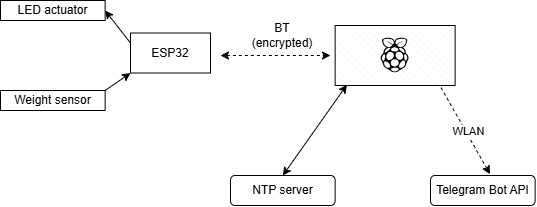
\includegraphics[width=\textwidth]{images/system_architecture.png}
	\caption{System architecture}
	\label{fig:architecture}
\end{figure}

The intake schedule is managed on the Raspberry Pi. For each intake time it
contains the medications, their quantity and the resulting target weight. Only
the intake times and target weights of the current day are transmitted to the
ESP32 via Bluetooth together with the current time at start-up; the names of the medications remain on the
Raspberry Pi and are only used for the Telegram reminder. The
evaluation of the intake takes place locally on the ESP32, so that the LED
display also works when the connection is interrupted. The software is
implemented in C according to MISRA C and is divided into several threads.

\subsection{Software modules}

\subsubsection{Safety related modules}
	\begin{enumerate}
		\item Weight measurement (ESP32): \\
			Description: Reads the load cell via the HX711, converts the raw
			values into grams, smooths them and checks them for plausibility.
			The calibration factor and the tare offset of the empty container
			are determined once during commissioning using a reference weight
			and are stored in non-volatile memory (NVS). At start-up, the
			module checks whether the filling of the container corresponds to
			the sum of the target weights of the day. \\
			Functions: weight\_read(), weight\_calibrate(),
			weight\_check\_filling() \\
			Data: Raw value, calibration factor, tare offset, weight in grams \\
			Requirements see: \ref{req.2.1}--\ref{req.2.5}, \ref{req.2.7}--\ref{req.2.10}

		\item Dose evaluation and intake monitoring (ESP32): \\
			Description: Creates a table of the expected weights for the day
			from the schedule. In each cycle, it compares the measured weight
			with the expected weight after the last due intake. If it matches,
			the dose is considered taken, also outside an intake window (late
			intake). Otherwise, within an intake window the dose is not yet
			taken or a wrong amount was removed. Outside an intake window, the
			deviation is detected as a missed dose or an unscheduled removal. \\
			Functions: table\_create(), dose\_evaluate() \\
			Data: Table of expected weights, tolerance, status \\
			Requirements see: \ref{req.1.6}--\ref{req.1.8}, \ref{req.2.6}, \ref{req.2.11}--\ref{req.2.13}, \ref{req.3.2}, \ref{req.3.3}

		\item LED status display (ESP32): \\
			Description: Displays the status via the RGB LED and tests all
			three colour channels at program start. \\
			Functions: led\_set\_status(), led\_self\_test() \\
			Data: Current status \\
			Requirements see: \ref{req.1.6}--\ref{req.1.8}, \ref{req.2.6}, \ref{req.2.10}, \ref{req.2.12}, \ref{req.2.13}, \ref{req.3.3}

		\item Intake schedule and time control (Raspberry Pi): \\
			Description: Reads the intake schedule from a configuration file
			maintained by the nursing staff and calculates the target weight
			of each intake time (quantity $\times$ weight of one tablet).
			Transmits the intake times and target weights to the ESP32 and
			triggers the push notification at the intake time, which lists the
			medications and their quantity. The time is synchronised via NTP. \\
			Functions: schedule\_load(), schedule\_check\_due() \\
			Data: Configuration file (medication names, weight of one tablet,
			intake times, quantity), calculated target weights, system time \\
			Requirements see: \ref{req.1.1}--\ref{req.1.5}, \ref{req.1.9}--
			\ref{req.1.11}, \ref{req.4.6}
	\end{enumerate}

\subsubsection{Security related modules}
	\begin{enumerate}
		\item Bluetooth communication and encryption (ESP32 and
		Raspberry Pi): \\
			Description: Establishes the connection, performs an ECDHE key
			exchange and encrypts all messages with AES-GCM. A sequence number
			protects against replay attacks. The Raspberry Pi only connects to
			the BLE address of the ESP32 stored in its configuration file.
			Both devices hold a common pre-shared key (PSK), which is stored
			once during commissioning. The session key is derived from the
			ECDHE shared secret and the PSK, so that only the two known devices
			can communicate with each other. \\
			Functions: bt\_send(), bt\_receive() \\
			Data: Pre-shared key, BLE address of the partner, session key,
			sequence counter, message buffer \\
			Requirements see: \ref{req.3.1}--\ref{req.3.5}, \ref{req.4.1}--\ref{req.4.3},
			\ref{req.4.7}--\ref{req.4.9}

		\item Telegram connection (Raspberry Pi): \\
			Description: Sends reminders and warnings via the Telegram Bot API
			over HTTPS and verifies the server certificate. Before the first NTP
			synchronisation, the last system time saved at shutdown is used for
			this check. \\
			Functions: telegram\_send() \\
			Data: Bot token, chat ID, message text (medication names and
			quantity) \\
			Requirements see: \ref{req.1.2}, \ref{req.1.10}, \ref{req.1.11}, \ref{req.2.6}, \ref{req.2.10}, \ref{req.2.13}, \ref{req.3.5}, \ref{req.4.5}, \ref{req.4.10}
	\end{enumerate}

\subsubsection{Modules with no influence on safety and security}
	\begin{enumerate}
		\item System start and logging (ESP32 and Raspberry Pi): \\
			Description: Initialises the hardware and modules, starts the
			threads and outputs status messages without health data. \\
			Functions: app\_main() or main() \\
			Requirements see: \ref{req.4.4}, \ref{req.5.1}--\ref{req.5.4}
	\end{enumerate}

\subsection{Libraries}

ESP-IDF with FreeRTOS (ESP32)
	\begin{itemize}
		\item xTaskCreate(pvTaskCode, pcName, usStackDepth, pvParameters,
		uxPriority, pxCreatedTask) creates a thread.
		\item gpio\_set\_level(gpio\_num, level) and gpio\_get\_level(gpio\_num)
		control the HX711 and switch the colour channels of the RGB LED on and
		off.
		\item esp\_timer\_start\_periodic(timer, period) starts the periodic
		timer for the measurement interval and the intake time window.
		\item portENTER\_CRITICAL(mux) and portEXIT\_CRITICAL(mux) disable and
		re-enable interrupts while the HX711 is being read.
		\item ble\_gatts\_notify\_custom(conn\_handle, chr\_val\_handle, om) from
		NimBLE sends a message to the Raspberry Pi.
		\item nvs\_set\_blob(handle, key, value, length) and nvs\_get\_blob(handle,
		key, out\_value, length) store and read the calibration data in the
		non-volatile memory.
		\item rtc\_gpio\_hold\_en(gpio\_num) keeps the red LED switched on
		during deep sleep if a missed dose is displayed.
		\item esp\_deep\_sleep\_start() puts the ESP32 into deep sleep mode after
		the last intake window of the day. It only wakes up when the reset
		button (EN) is pressed.
	\end{itemize}

mbedTLS (ESP32 and Raspberry Pi)
	\begin{itemize}
		\item mbedtls\_ecdh\_calc\_secret(ctx, olen, buf, blen, f\_rng, p\_rng)
		computes the shared secret during the key exchange.
		\item mbedtls\_gcm\_crypt\_and\_tag(ctx, mode, length, iv, iv\_len, add,
		add\_len, input, output, tag\_len, tag) encrypts a message.
		\item mbedtls\_gcm\_auth\_decrypt(ctx, length, iv, iv\_len, add, add\_len,
		tag, tag\_len, input, output) decrypts a message and verifies its
		integrity.
		\item mbedtls\_hkdf(md, salt, salt\_len, ikm, ikm\_len, info, info\_len,
		okm, okm\_len) derives the session key from the ECDHE shared secret
		and the pre-shared key.
	\end{itemize}

Raspberry Pi
	\begin{itemize}
		\item pthread\_create(thread, attr, start\_routine, arg) creates a
		thread.
		\item curl\_easy\_perform(handle) from libcurl sends the HTTPS request
		to the Telegram Bot API.
		\item clock\_gettime(clock\_id, tp) reads the system time synchronised
		via NTP.
		\item WriteValue(value, options) and StartNotify() are methods of the
		BlueZ D-Bus interface org.bluez.GattCharacteristic1 and send messages
		to the ESP32 or enable reception.
	\end{itemize}

For Bluetooth, the NimBLE stack included in ESP-IDF is used on the ESP32 and
BlueZ is used on the Raspberry Pi.

The libraries used are available at ESP-IDF
\url{https://github.com/espressif/esp-idf}, mbedTLS
\url{https://github.com/Mbed-TLS/mbedtls}, BlueZ
\url{https://git.kernel.org/pub/scm/bluetooth/bluez.git} and libcurl
\url{https://curl.se/libcurl/}.

\subsection{Interrupts}

The ESP32 uses a timer interrupt for the measurement interval and the intake
time window, as well as interrupts from the Bluetooth stack when messages are
received. The interrupt routines only notify the responsible thread. The
thread priorities follow the rule of safety before communication before
logging (see Table~\ref{tab:prio}).

\begin{table}[H]
	\centering
	\begin{tabular}{|l|c|}
		\hline
		Thread & Priority \\
		\hline
		Weight measurement & high \\
		Dose evaluation and LED status display & high \\
		Bluetooth communication & medium \\
		Heartbeat & medium \\
		Logging & low \\
		\hline
	\end{tabular}
	\caption{Thread priorities on the ESP32}
	\label{tab:prio}
\end{table}

Reading the HX711 is time-critical, as it enters power-down mode if the clock
line remains HIGH for too long (more than 60 µs). It is therefore performed
without interruption by other interrupts.

On the Raspberry Pi, interrupts are managed by the operating system (Linux).
Bluetooth communication, time control and the Telegram connection each run
in their own POSIX thread.

\subsection{Pinout}

The load cell is connected to the ESP32 via the HX711. The RGB LED is
connected directly to three GPIO pins that are configured as digital outputs.
Since the KY-009 module has no built-in series resistors, a series resistor is
placed in each colour line. The resistors are calculated using
$R = (3.3\,\mathrm{V} - U_F) / I$. With a forward voltage $U_F$ of
approximately 1.8~V for red and 2.8~V for green and blue, 220~$\Omega$ is
chosen for red (approx.\ 7~mA) and 160~$\Omega$ for green and blue
(approx.\ 3~mA). These currents are sufficient for a status display and stay
well below the maximum current of an ESP32 GPIO pin. Since there are variants of the module in which red
and green are swapped, the pin assignment is checked individually before the
final wiring (source
\url{https://arduinomodules.info/ky-009-rgb-full-color-led-smd-module/}).
Figure~\ref{fig:wiring} shows the complete wiring, Tables~\ref{tab:pinout-loadcell}--\ref{tab:pinout-led} list the individual connections.

\begin{figure}[H]
  \centering
  \resizebox{\textwidth}{!}{%
  \begin{tikzpicture}[
      font=\small,
      dev/.style={draw, thick, fill=gray!8, minimum width=24mm, align=center},
      pin/.style={font=\scriptsize, inner sep=1pt},
      w/.style={line width=1.2pt},
      res/.style={draw, fill=white, minimum width=9mm, minimum height=3.5mm, inner sep=0pt, font=\scriptsize}
    ]
    % y positions of the four rows
    \def\ya{3.0} \def\yb{2.4} \def\yc{1.8} \def\yd{1.2}

    % --- devices ---
    \node[dev, minimum height=30mm] (lc)  at (-9.6,2.1) {Load cell\\(100\,g)};
    \node[dev, minimum height=30mm, minimum width=26mm, label={[font=\small\bfseries]above:HX711}] (hx) at (-4.8,2.1) {};
    \node[dev, minimum height=30mm, minimum width=34mm, label={[font=\small\bfseries]above:ESP32}] (esp) at (0,2.1) {};
    \node[dev, minimum height=30mm, minimum width=30mm, label={[font=\small\bfseries]above:KY-009 (RGB LED)}] (led) at (6.8,2.1) {};

    % --- HX711 pins ---
    \foreach \y/\n in {\ya/E+, \yb/E$-$, \yc/A$-$, \yd/A+}
      \node[pin, anchor=west] at ($(hx.west |- 0,\y)$) {\n};
    \foreach \y/\n in {\ya/VCC, \yb/GND, \yc/DT, \yd/SCK}
      \node[pin, anchor=east] at ($(hx.east |- 0,\y)$) {\n};
    % --- ESP32 pins ---
    \foreach \y/\n in {\ya/3V3, \yb/GND, \yc/GPIO\,19, \yd/GPIO\,18}
      \node[pin, anchor=west] at ($(esp.west |- 0,\y)$) {\n};
    \foreach \y/\n in {\ya/GPIO\,25, \yb/GPIO\,26, \yc/GPIO\,27, \yd/GND}
      \node[pin, anchor=east] at ($(esp.east |- 0,\y)$) {\n};
    % --- KY-009 pins ---
    \foreach \y/\n in {\ya/R, \yb/G, \yc/B, \yd/$-$}
      \node[pin, anchor=west] at ($(led.west |- 0,\y)$) {\n};

    % --- load cell -> HX711 (wire colours of the load cell) ---
    \draw[w, red]        ($(lc.east |- 0,\ya)$) -- node[pin, above, black]{red}   ($(hx.west |- 0,\ya)$);
    \draw[w, black]      ($(lc.east |- 0,\yb)$) -- node[pin, above]{black}        ($(hx.west |- 0,\yb)$);
    \draw[w, gray!50]    ($(lc.east |- 0,\yc)$) -- node[pin, above, black]{white} ($(hx.west |- 0,\yc)$);
    \draw[w, green!60!black] ($(lc.east |- 0,\yd)$) -- node[pin, above, black]{green} ($(hx.west |- 0,\yd)$);

    % --- HX711 -> ESP32 ---
    \draw[w, red]        ($(hx.east |- 0,\ya)$) -- ($(esp.west |- 0,\ya)$);
    \draw[w, black]      ($(hx.east |- 0,\yb)$) -- ($(esp.west |- 0,\yb)$);
    \draw[w, orange]     ($(hx.east |- 0,\yc)$) -- node[pin, above, black]{data}  ($(esp.west |- 0,\yc)$);
    \draw[w, violet]     ($(hx.east |- 0,\yd)$) -- node[pin, above, black]{clock} ($(esp.west |- 0,\yd)$);

    % --- ESP32 -> series resistors -> KY-009 ---
    \foreach \y/\c/\r in {\ya/red/220, \yb/green!60!black/160, \yc/blue/160} {
      \draw[w, \c] ($(esp.east |- 0,\y)$) -- ($(led.west |- 0,\y)$);
      \node[res] at ($(esp.east |- 0,\y)!0.5!(led.west |- 0,\y)$) {\r\,$\Omega$};
    }
    \draw[w, black] ($(esp.east |- 0,\yd)$) -- node[pin, above]{common cathode} ($(led.west |- 0,\yd)$);
  \end{tikzpicture}
  }
  \caption{Wiring of the load cell, HX711, ESP32 and RGB LED}
  \label{fig:wiring}
\end{figure}

\begin{table}[H]
	\centering
	\begin{tabular}{|l|l|}
		\hline
		Load cell (wire) & HX711 \\
		\hline
		Red & E+ \\
		Black & E$-$ \\
		White & A$-$ \\
		Green & A+ \\
		\hline
	\end{tabular}
	\caption{Pinout load cell and HX711}
	\label{tab:pinout-loadcell}
\end{table}

\begin{table}[H]
	\centering
	\begin{tabular}{|l|l|}
		\hline
		ESP32 pin & HX711 \\
		\hline
		3V3 & VCC \\
		GND & GND \\
		GPIO 19 & DT (data) \\
		GPIO 18 & SCK (clock) \\
		\hline
	\end{tabular}
	\caption{Pinout ESP32 and HX711}
	\label{tab:pinout-hx711}
\end{table}

\begin{table}[H]
	\centering
	\begin{tabular}{|l|l|}
		\hline
		ESP32 pin & KY-009 \\
		\hline
		GPIO 25 (via 220~$\Omega$) & R (red) \\
		GPIO 26 (via 160~$\Omega$) & G (green) \\
		GPIO 27 (via 160~$\Omega$) & B (blue) \\
		GND & $-$ (common cathode) \\
		\hline
	\end{tabular}
	\caption{Pinout ESP32 and RGB LED (KY-009)}
	\label{tab:pinout-led}
\end{table}